\documentclass[onecolumn, compsoc,9pt]{IEEEtran}
\usepackage{etex}
\usepackage{amssymb,amsfonts,amsmath,amsthm}
\usepackage{graphicx}
\usepackage[usenames,x11names, dvipsnames, svgnames]{xcolor}
\usepackage{amsmath,amssymb}
\usepackage{dsfont}
\usepackage{amsfonts}
\usepackage{mathrsfs}
\usepackage{texshade}
\usepackage{hyperref}
\hypersetup{
  colorlinks=true,
  linkcolor=black,
  citecolor=black,
  filecolor=black,
  urlcolor=DodgerBlue4,
  breaklinks=false,
  % linkbordercolor=red,% hyperlink borders will be red
  % pdfborderstyle={/S/U/W 1}% border style will be underline of width 1pt
}
\usepackage{array}
\usepackage{xr}
\usepackage{verbatim}
\usepackage{multirow}
\usepackage{longtable}
% \usepackage[T1,euler-digits]{eulervm}
% \usepackage{times}
% \usepackage{pxfonts}
\usepackage{tikz}
\usepackage{pgfplots}
\usetikzlibrary{shapes,calc,shadows,fadings,arrows,decorations.pathreplacing,automata,positioning}
\usetikzlibrary{external}
\usetikzlibrary{decorations.text}
\usepgfplotslibrary{colorbrewer} 

\tikzexternalize[prefix=./Figures/External/]% activate externalization!
\tikzexternaldisable
% \addtolength{\voffset}{.1in}  
\usepackage{geometry}
\geometry{a4paper, left=.65in,right=.65in,top=.8in,bottom=0.7in}

\addtolength{\textwidth}{-.1in}    
\addtolength{\hoffset}{.05in}    
\addtolength{\textheight}{.1in}    
\addtolength{\footskip}{0in}    
\usepackage{rotating}
\definecolor{nodecol}{RGB}{240,240,220}
\definecolor{nodeedge}{RGB}{240,240,225}
\definecolor{edgecol}{RGB}{130,130,130}
\tikzset{%
  fshadow/.style={      preaction={
      fill=black,opacity=.3,
      path fading=circle with fuzzy edge 20 percent,
      transform canvas={xshift=1mm,yshift=-1mm}
    }} 
}
\usetikzlibrary{pgfplots.dateplot}
\usetikzlibrary{patterns}
\usetikzlibrary{decorations.markings}
\usepackage{fancyhdr}
\usepackage{mathtools}
\usepackage{datetime}
\usepackage[group-separator={,}]{siunitx}
%% ## Equation Space Control---------------------------
\def\EQSP{3pt}
\newcommand{\mltlne}[2][\EQSP]{\begingroup\setlength\abovedisplayskip{#1}\setlength\belowdisplayskip{#1}\begin{equation}\begin{multlined} #2 \end{multlined}\end{equation}\endgroup\noindent}
\newcommand{\cgather}[2][\EQSP]{\begingroup\setlength\abovedisplayskip{#1}\setlength\belowdisplayskip{#1}\begin{gather} #2 \end{gather}\endgroup\noindent}
\newcommand{\cgathers}[2][\EQSP]{\begingroup\setlength\abovedisplayskip{#1}\setlength\belowdisplayskip{#1}\begin{gather*} #2 \end{gather*}\endgroup\noindent}
\newcommand{\calign}[2][\EQSP]{\begingroup\setlength\abovedisplayskip{#1}\setlength\belowdisplayskip{#1}\begin{align} #2 \end{align}\endgroup\noindent}
\newcommand{\caligns}[2][\EQSP]{\begingroup\setlength\abovedisplayskip{#1}\setlength\belowdisplayskip{#1}\begin{align*} #2 \end{align*}\endgroup\noindent}
\newcommand{\mnp}[2]{\begin{minipage}{#1}#2\end{minipage}} 
%% COLOR DEFS------------------------------------------
\newtheorem{thm}{Theorem}
\newtheorem{cor}{Corollary}
\newtheorem{lem}{Lemma}
\newtheorem{prop}{Proposition}
\newtheorem{defn}{Definition}
\newtheorem{exmpl}{Example}
\newtheorem{rem}{Remark}
\newtheorem{notn}{Notation}
%% ------------PROOF INCLUSION -----------------
\def\NOPROOF{Proof omitted.}
\newif\ifproof
\prooffalse % or \draftfalse
\newcommand{\Proof}[1]{
  \ifproof
  \begin{IEEEproof}
    #1\end{IEEEproof}
  \else
  \NOPROOF
  \fi
}
%% ------------ -----------------
\newcommand{\DETAILS}[1]{#1}
%% ------------ -----------------
% color commands------------------------
\newcommand{\etal}{\textit{et} \mspace{3mu} \textit{al.}}
% \renewcommand{\algorithmiccomment}[1]{$/** $ #1 $ **/$}
\newcommand{\vect}[1]{\textbf{\textit{#1}}}
\newcommand{\figfont}{\fontsize{8}{8}\selectfont\strut}
\newcommand{\hlt}{ \bf \sffamily \itshape\color[rgb]{.1,.2,.45}}
\newcommand{\pitilde}{\widetilde{\pi}}
\newcommand{\Pitilde}{\widetilde{\Pi}}
\newcommand{\bvec}{\vartheta}
\newcommand{\algo}{\textrm{\bf\texttt{GenESeSS}}\xspace}
\newcommand{\xalgo}{\textrm{\bf\texttt{xGenESeSS}}\xspace}
\newcommand{\FNTST}{\bf }
\newcommand{\FNTED}{\color{darkgray} \scriptsize $\phantom{.}$}
\renewcommand{\baselinestretch}{.95}
\newcommand{\sync}{\otimes}
\newcommand{\psync}{\hspace{3pt}\overrightarrow{\hspace{-3pt}\sync}}
% \newcommand{\psync}{\raisebox{-4pt}{\begin{tikzpicture}\node[anchor=south] (A) {$\sync$};
%   \draw [->,>=stealth] ([yshift=-2pt, xshift=2pt]A.north west) -- ([yshift=-2pt]A.north east); %\end{tikzpicture}}}
\newcommand{\base}[1]{\llbracket #1 \rrbracket}
\newcommand{\nst}{\textrm{\sffamily\textsc{Numstates}}}
\newcommand{\HA}{\boldsymbol{\mathds{H}}}
\newcommand{\eqp}{ \vartheta }
\newcommand{\entropy}[1]{\boldsymbol{h}\left ( #1 \right )}
\newcommand{\norm}[1]{\left\lVert #1 \right\rVert}%
\newcommand{\abs}[1]{\left\lvert #1 \right\rvert}%
\newcommand{\absB}[1]{\big\lvert #1 \big\rvert}%
% #############################################################
% #############################################################
% PREAMBLE ####################################################
% #############################################################
% #############################################################
% \usepackage{pnastwoF}      
\DeclareMathOperator*{\argmax}{argmax}
\DeclareMathOperator*{\argmin}{arg\,min}
\DeclareMathOperator*{\expect}{\mathbf{E}}
\DeclareMathOperator*{\var}{\mathbf{Var}}

\newcommand{\ND}{ \mathcal{N}  }
\usepackage[linesnumbered,ruled,vlined,noend]{algorithm2e}
\newcommand{\captionN}[1]{\caption{\color{darkgray} \sffamily \fontsize{9}{10}\selectfont #1  }}
\newcommand{\btl}{\ \textbf{\small\sffamily bits/letter}}
\usepackage{txfonts}
% \usepackage{ccfonts}
%%% save defaults
\renewcommand{\rmdefault}{phv} % Arial
\renewcommand{\sfdefault}{phv} % Arial
\edef\keptrmdefault{\rmdefault}
\edef\keptsfdefault{\sfdefault}
\edef\keptttdefault{\ttdefault}

% \usepackage{kerkis}
\usepackage[OT1]{fontenc}
\usepackage{concmath}
% \usepackage[T1]{eulervm} 
% \usepackage[OT1]{fontenc}
%%% restore defaults
\edef\rmdefault{\keptrmdefault}
\edef\sfdefault{\keptsfdefault}
\edef\ttdefault{\keptttdefault}
\tikzexternalenable
% ##########################################################
\tikzfading[name=fade out,
inner color=transparent!0,
outer color=transparent!100]
% ###################################
\newcommand{\xtitaut}[2]{
  \noindent\mnp{\textwidth}{
    \mnp{\textwidth}{\raggedright\Huge \bf \sffamily #1}

    \vskip 1em

    {\bf \sffamily #2}
  }
  \vskip 2em
}
% ###################################
% ###################################
\tikzset{wiggle/.style={decorate, decoration={random steps, amplitude=10pt}}}
\usetikzlibrary{decorations.pathmorphing}
\pgfdeclaredecoration{Snake}{initial}
{
  \state{initial}[switch if less than=+.625\pgfdecorationsegmentlength to final,
  width=+.3125\pgfdecorationsegmentlength,
  next state=down]{
    \pgfpathmoveto{\pgfqpoint{0pt}{\pgfdecorationsegmentamplitude}}
  }
  \state{down}[switch if less than=+.8125\pgfdecorationsegmentlength to end down,
  width=+.5\pgfdecorationsegmentlength,
  next state=up]{
    \pgfpathcosine{\pgfqpoint{.25\pgfdecorationsegmentlength}{-1\pgfdecorationsegmentamplitude}}
    \pgfpathsine{\pgfqpoint{.25\pgfdecorationsegmentlength}{-1\pgfdecorationsegmentamplitude}}
  }
  \state{up}[switch if less than=+.8125\pgfdecorationsegmentlength to end up,
  width=+.5\pgfdecorationsegmentlength,
  next state=down]{
    \pgfpathcosine{\pgfqpoint{.25\pgfdecorationsegmentlength}{\pgfdecorationsegmentamplitude}}
    \pgfpathsine{\pgfqpoint{.25\pgfdecorationsegmentlength}{\pgfdecorationsegmentamplitude}}
  }
  \state{end down}[width=+.3125\pgfdecorationsegmentlength,
  next state=final]{
    \pgfpathcosine{\pgfqpoint{.15625\pgfdecorationsegmentlength}{-.5\pgfdecorationsegmentamplitude}}
    \pgfpathsine{\pgfqpoint{.15625\pgfdecorationsegmentlength}{-.5\pgfdecorationsegmentamplitude}}
  }
  \state{end up}[width=+.3125\pgfdecorationsegmentlength,
  next state=final]{
    \pgfpathcosine{\pgfqpoint{.15625\pgfdecorationsegmentlength}{.5\pgfdecorationsegmentamplitude}}
    \pgfpathsine{\pgfqpoint{.15625\pgfdecorationsegmentlength}{.5\pgfdecorationsegmentamplitude}}
  }
  \state{final}{\pgfpathlineto{\pgfpointdecoratedpathlast}}
}
% ###################################
% ###################################
\newcolumntype{L}[1]{>{\rule{0pt}{2ex}\raggedright\let\newline\\\arraybackslash\hspace{0pt}}m{#1}}
\newcolumntype{C}[1]{>{\rule{0pt}{2ex}\centering\let\newline\\\arraybackslash\hspace{0pt}}m{#1}}
\newcolumntype{R}[1]{>{\rule{0pt}{2ex}\raggedleft\let\newline\\\arraybackslash\hspace{0pt}}m{#1}}



% ################################################
% ################################################
% ################################################
% ################################################
\def\DISCLOSURE#1{\def\disclosure{#1}}
\DISCLOSURE{\raisebox{15pt}{$\phantom{XxxX}$This sheet contains proprietary information 
    not to be released to third parties except for the explicit purpose of evaluation.}
}
% ####################################
\newcommand{\set}[1]{\left\{ #1 \right\}}
\newcommand{\paren}[1]{\left( #1 \right)}
\newcommand{\bracket}[1]{\left[ #1 \right]}
% \newcommand{\norm}[1]{\left\Vert #1 \right\Vert}
\newcommand{\nrm}[1]{\left\llbracket{#1}\right\rrbracket}
\newcommand{\parenBar}[2]{\paren{#1\,{\left\Vert\,#2\right.}}}
\newcommand{\parenBarl}[2]{\paren{\left.#1\,\right\Vert\,#2}}
\newcommand{\ie}{$i.e.$\xspace}
\newcommand{\addcitation}{\textcolor{black!50!red}{\textbf{ADD CITATION}}}
\newcommand{\subtochange}[1]{{\color{black!50!green}{#1}}}
\newcommand{\tobecompleted}{{\color{black!50!red}TO BE COMPLETED.}}


\newcommand{\pIn}{\mathscr{P}_{\textrm{in}}}
\newcommand{\pOut}{\mathscr{P}_{\textrm{out}}}
\newcommand{\aIn}[1][\Sigma]{#1_{\textrm{in}}}
\newcommand{\aOut}[1][\Sigma]{#1_{\textrm{out}}}
\newcommand{\xin}[1]{#1_{\textrm{in}}}
\newcommand{\xout}[1]{#1_{\textrm{out}}}

\newcommand{\R}{\mathbb{R}} % Set of real numbers
\newcommand{\F}[1][]{\mathcal{F}_{#1}}
\newcommand{\SR}{\mathcal{S}} % Semiring of sets
\newcommand{\RR}{\mathcal{R}} % Ring of sets
\newcommand{\N}{\mathbb{N}} % Set of natural numbers (0 included)


\newcommand{\Pp}[1][n]{\mathscr{P}^+_{#1}}
\renewcommand{\entropy}[1]{\boldsymbol{h}\left ( #1 \right )}



\makeatletter
\pgfdeclarepatternformonly[\hatchdistance,\hatchthickness]{flexible hatch}
{\pgfqpoint{0pt}{0pt}}
{\pgfqpoint{\hatchdistance}{\hatchdistance}}
{\pgfpoint{\hatchdistance-1pt}{\hatchdistance-1pt}}%
{
  \pgfsetcolor{\tikz@pattern@color}
  \pgfsetlinewidth{\hatchthickness}
  \pgfpathmoveto{\pgfqpoint{0pt}{0pt}}
  \pgfpathlineto{\pgfqpoint{\hatchdistance}{\hatchdistance}}
  \pgfusepath{stroke}
}
\makeatother

\pgfdeclarepatternformonly{north east lines wide}%
{\pgfqpoint{-1pt}{-1pt}}%
{\pgfqpoint{10pt}{10pt}}%
{\pgfqpoint{9pt}{9pt}}%
{
  \pgfsetlinewidth{0.7pt}
  \pgfpathmoveto{\pgfqpoint{0pt}{0pt}}
  \pgfpathlineto{\pgfqpoint{9.1pt}{9.1pt}}
  \pgfusepath{stroke}
}

\pgfdeclarepatternformonly{north west lines wide}%
{\pgfqpoint{-1pt}{-1pt}}%
{\pgfqpoint{10pt}{10pt}}%
{\pgfqpoint{9pt}{9pt}}%
{
  \pgfsetlinewidth{0.7pt}
  \pgfpathmoveto{\pgfqpoint{0pt}{9pt}}
  \pgfpathlineto{\pgfqpoint{9.1pt}{-0.1pt}}
  \pgfusepath{stroke}
}
\makeatletter

\pgfdeclarepatternformonly[\hatchdistance,\hatchthickness]{flexible hatchB}
{\pgfqpoint{0pt}{\hatchdistance}}
{\pgfqpoint{\hatchdistance}{0pt}}
{\pgfpoint{1pt}{\hatchdistance-1pt}}%
{
  \pgfsetcolor{\tikz@pattern@color}
  \pgfsetlinewidth{\hatchthickness}
  \pgfpathmoveto{\pgfqpoint{0pt}{\hatchdistance}}
  \pgfpathlineto{\pgfqpoint{\hatchdistance}{0pt}}
  \pgfusepath{stroke}
}    \makeatother


\def\TPR{\textrm{TPR}\xspace}
\def\TNR{\textrm{TNR}\xspace}
\def\FPR{\textrm{FPR}\xspace}
\def\PPV{\textrm{PPV}\xspace}

\usetikzlibrary{arrows.meta}
\usetikzlibrary{decorations.pathreplacing,shapes.misc}
\usepgfplotslibrary{fillbetween}
%usepackage{tikz-network}
\usetikzlibrary{shapes.geometric}
\usetikzlibrary{math}
\usepgfplotslibrary{colorbrewer} 

\usepackage{textcomp}
\usepackage{colortbl}
\usepackage{array}
\usepackage{courier} 
\usepackage{wrapfig}
\usepackage{pifont}
\usetikzlibrary{chains,backgrounds}
\usetikzlibrary{intersections}
\usetikzlibrary{pgfplots.groupplots}
\usepgfplotslibrary{fillbetween} 
\usetikzlibrary{arrows.meta}
\usepackage{pgfplotstable}
\usepackage[super,compress,sort,comma]{natbib}
%\usepackage{natbib}
\usepackage{setspace}
\usetikzlibrary{math}
\usetikzlibrary{matrix}
\usepackage{xstring}
\usepackage{xspace}
\usepackage{flushend}
\makeatletter
\renewcommand\section{\@startsection {section}{1}{\z@}%
  {-2ex \@plus -1ex \@minus -.2ex}%
  {1ex \@plus.1ex}%
  {\Large\bfseries\scshape}}
\renewcommand\subsection{\@startsection {section}{1}{\z@}%
  {-2ex \@plus -.25ex \@minus -.2ex}%
  {0.1ex \@plus.0ex}%
  {\fontsize{11}{10}\selectfont\bfseries\sffamily\color{black}}}
\renewcommand\subsubsection{\@startsection {section}{1}{\z@}%
  {0ex \@plus -.5ex \@minus -.2ex}%
  {0.0ex \@plus.5ex}%
  {\fontsize{9}{9}\selectfont\bfseries\itshape\sffamily\color{darkgray}}}
\renewcommand\paragraph{\@startsection {section}{1}{\z@}%
  {-.2ex \@plus -.5ex \@minus -.2ex}%
  {0.0ex \@plus.5ex}%
  {\fontsize{9}{9}\selectfont\itshape\sffamily\color{darkgray}}}
       
 
\makeatother
\makeatletter
\pgfdeclareradialshading[tikz@ball]{ball}{\pgfqpoint{-10bp}{10bp}}{%
  color(0bp)=(tikz@ball!30!white);
  color(9bp)=(tikz@ball!75!white);
  color(18bp)=(tikz@ball!90!black);
  color(25bp)=(tikz@ball!70!black);
  color(50bp)=(black)}
\makeatother
%\newcommand{\tball}[1][CadetBlue4]{${\color{#1}\Large\boldsymbol{\blacksquare}}$}
\renewcommand{\baselinestretch}{1}
%\renewcommand{\captionN}[1]{\caption{\color{CadetBlue4!50!black} \sffamily \fontsize{9}{10}\selectfont #1  }}
\tikzexternaldisable 
\parskip=6pt
\parindent=0pt
%\newcommand{\Mark}[1]{\textsuperscript{#1}}
\pagestyle{fancy}

\newcounter{Dcounter}
\setcounter{Dcounter}{1}
\newcommand{\DQS}[1]{\ifdraftQ
{\marginpar{\tikzexternaldisable \tikz{\node[rounded corners=5pt,draw=none,thick,fill=black!10,font=\sffamily\fontsize{7}{8}\selectfont] {\mnp{.45in} {\color{Red3}\raggedright  \#\theDcounter.~#1}}; }}}\stepcounter{Dcounter}\xspace
\fi}

\newcommand{\qn}[1][i]{\Phi_{#1}}
\newcommand{\D}[1][i]{\mathscr{D}\left ( {\Sigma_#1} \right ) }
\newcommand{\Dx}{\mathscr{D}}
\def\J{\mathds{J}}
\def\M{\omega}
\def\N{\mathds{N}}
\newcommand{\cp}[1][P]{\langle #1 \rangle}
\newcommand{\mem}[1]{\M_{#1}}


\makeatletter
\newcommand\transformxdimension[1]{
    \pgfmathparse{((#1/\pgfplots@x@veclength)+\pgfplots@data@scale@trafo@SHIFT@x)/10^\pgfplots@data@scale@trafo@EXPONENT@x}
}
\newcommand\transformydimension[1]{
    \pgfmathparse{((#1/\pgfplots@y@veclength)+\pgfplots@data@scale@trafo@SHIFT@y)/10^\pgfplots@data@scale@trafo@EXPONENT@y}
}
\makeatother

\parskip=6pt
\parindent=0pt


\pgfplotsset{
    discard if/.style 2 args={
        x filter/.code={
            \edef\tempa{\thisrow{#1}}
            \edef\tempb{#2}
            \ifx\tempa\tempb
                \def\pgfmathresult{inf}
            \fi
        }
    },
    discard if not/.style 2 args={
        x filter/.code={
            \edef\tempa{\thisrow{#1}}
            \edef\tempb{#2}
            \ifx\tempa\tempb
            \else
                \def\pgfmathresult{inf}
            \fi
        }
    }
  } 
\usepackage{textcomp}
\usepackage{subfigure}
\usepackage{stmaryrd}
\usetikzlibrary{chains,backgrounds}
\usetikzlibrary{intersections}
\usepgfplotslibrary{groupplots}
\usepackage{xstring}

\renewcommand{\baselinestretch}{.93}
\renewcommand{\captionN}[1]{\caption{\color{darkgray} \sffamily \fontsize{8}{10}\selectfont #1  }}
% ###################################
% \parskip=4pt
% \parindent=0pt

\begin{document}  

\def\TITLE{PTSD Analysis}
%\twocolumn[{% 
  \fontsize{20}{20}\selectfont \bf \sffamily
  \flushleft  \TITLE \\\footnotesize  \vspace{10pt}  \bf \sffamily 
  ZeD Lab@UChicago \texttt{(zed.uchicago.edu)}\\
  \vskip .5em
  Department of Medicince, University of Chicago, Chicago IL, USA
  \vskip 5em
  % 
%}]
 \vskip 1em


 \begin{table}[!ht]
   \centering
  \caption{AUC at 99\% Confidence}
\begin{tabular}{L{.65in}|L{.5in}|L{.5in}|L{.5in}|L{.5in}}\hline
 Problem & Confidence & Lower & Upper & Mean \\\hline
SCZ vs SAFF&0.99&0.83&0.88&0.85\\\hline
SCZ vs REST&0.99&0.84&0.87&0.86\\\hline
SCZ+SAFF vs REST&0.99&0.92&0.94&0.93\\\hline
\end{tabular}

\end{table}

\def\WDT{2in}
\begin{figure}[!ht]
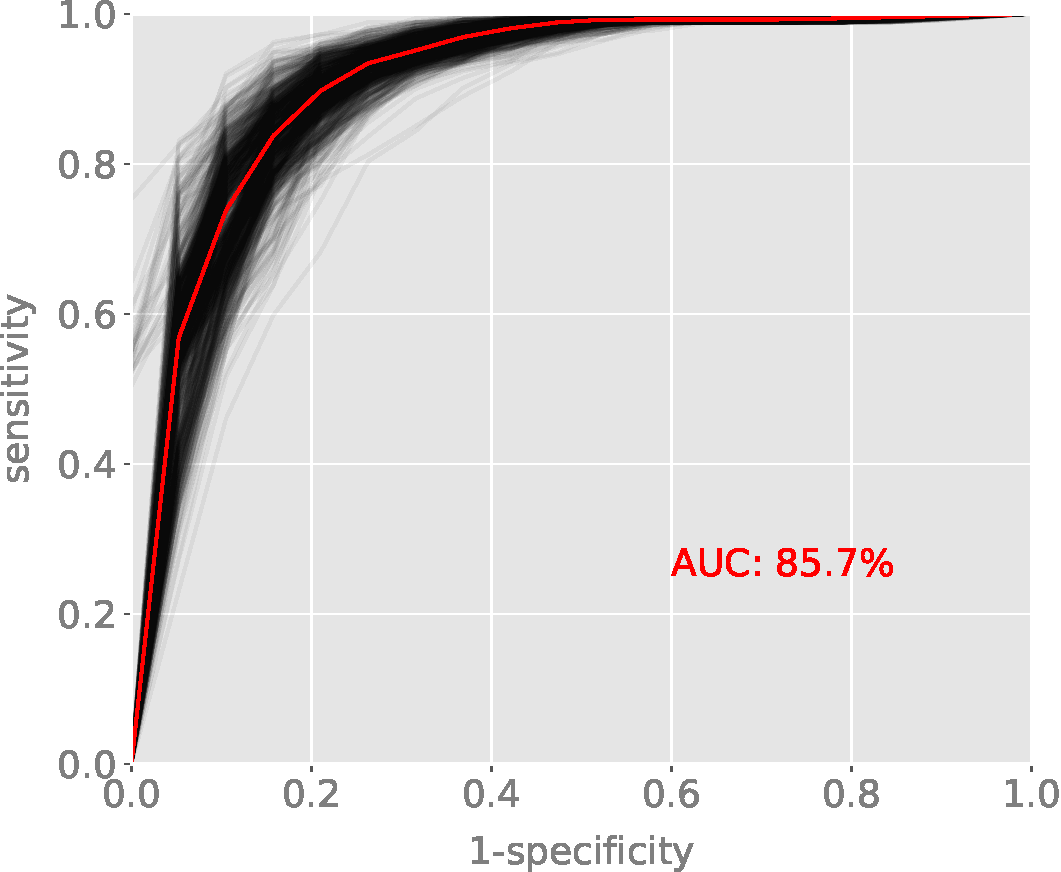
\includegraphics[width=\WDT]{Figures/sczVSall.pdf}
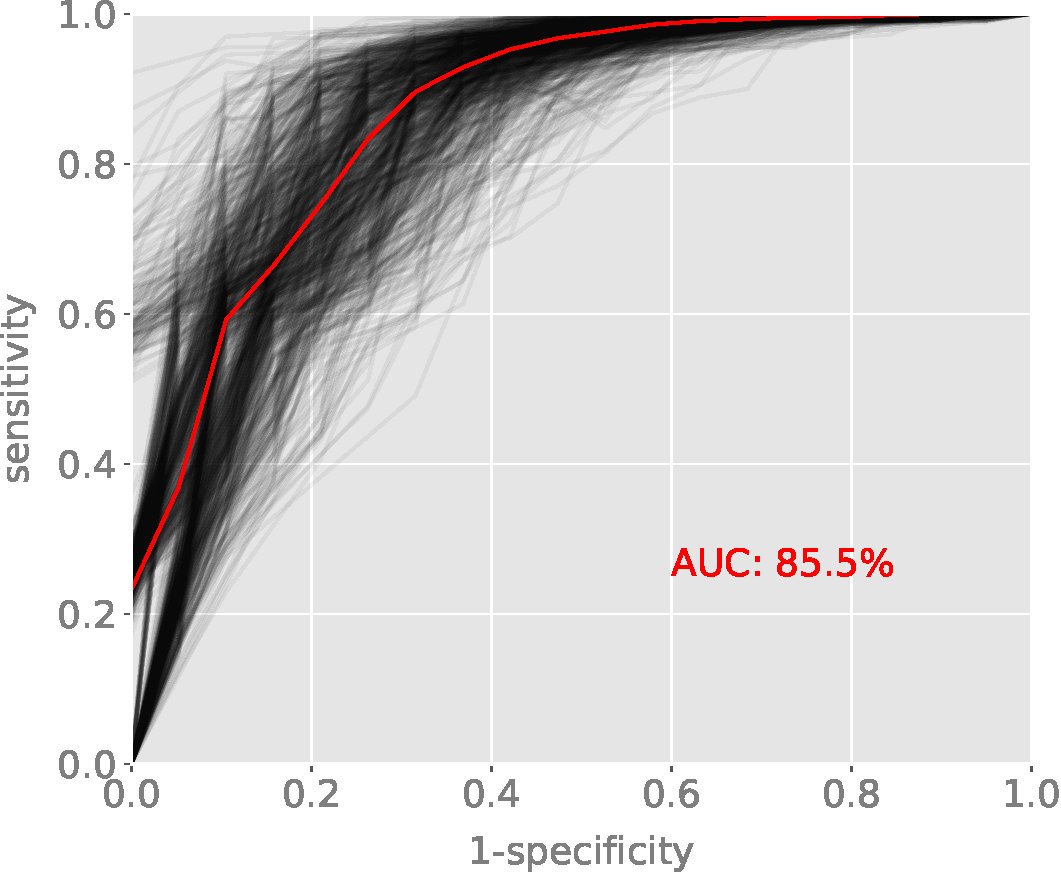
\includegraphics[width=\WDT]{Figures/sczVscaff.pdf}
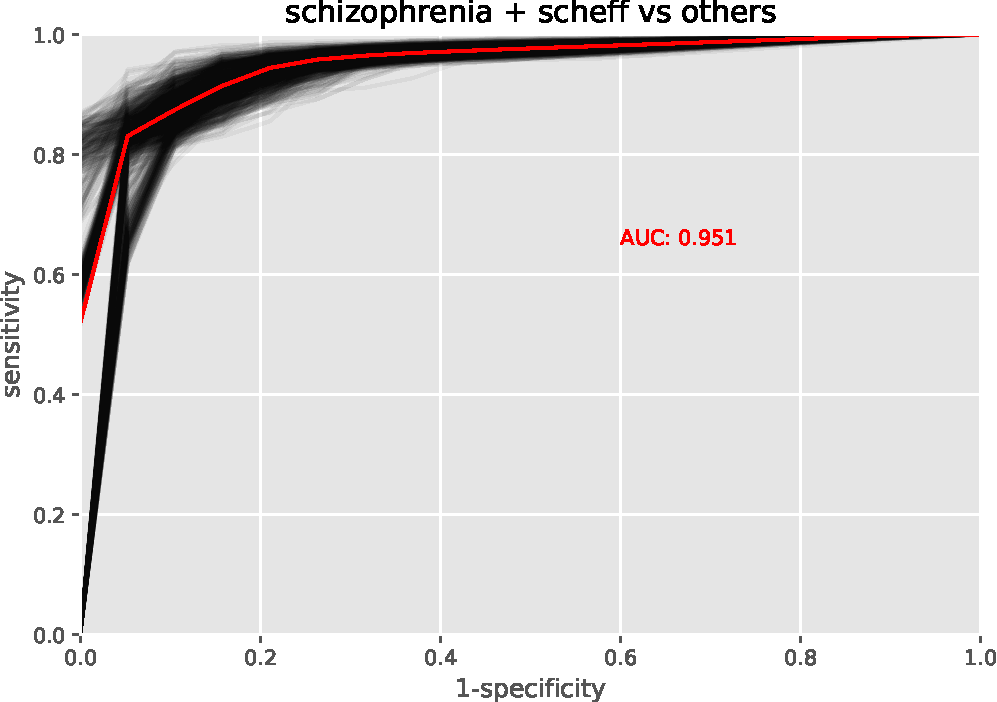
\includegraphics[width=\WDT]{Figures/sczsceff.pdf}
\end{figure}


\begin{tikzpicture}[font=\normalfont\sffamily\fontsize{8}{8}\selectfont]
\clip (-1.05in,-2.9in) rectangle (3.60in,1.1in);
  
\def\WDT{2in}
\node[] (a) at (0,0) {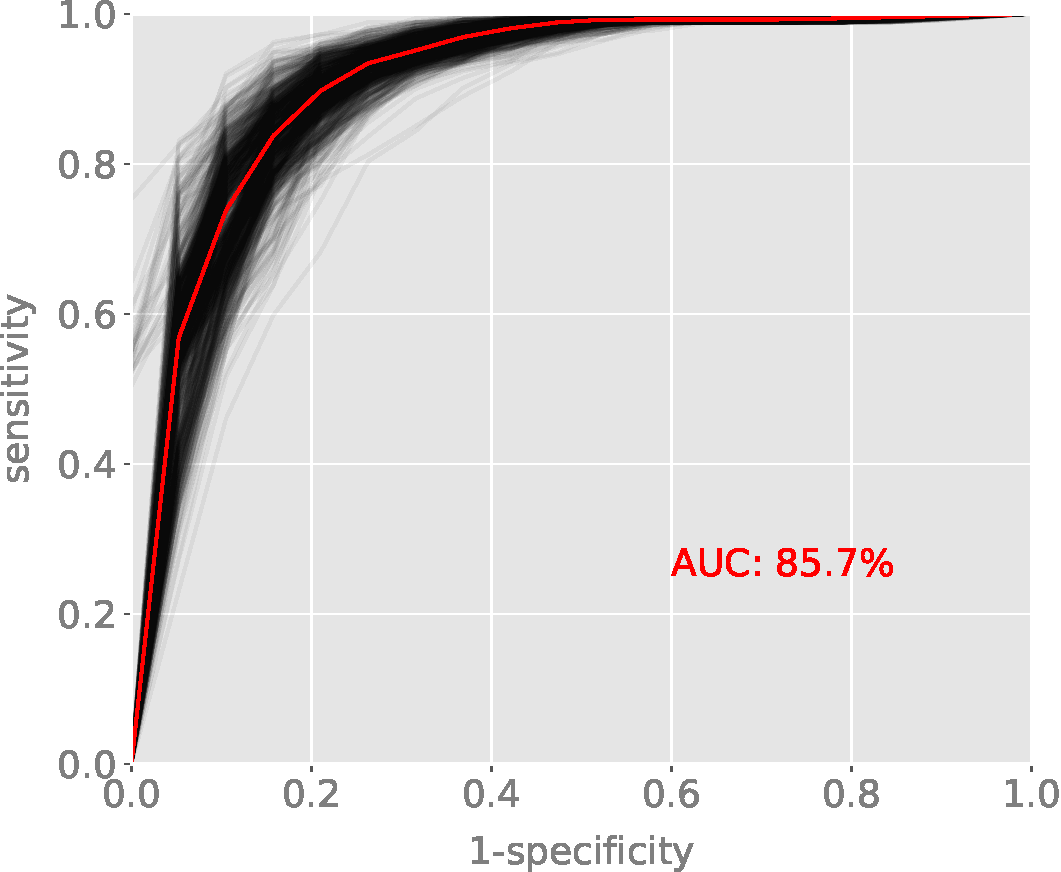
\includegraphics[width=\WDT]{Figures/sczVSall.pdf}};
\node[anchor=west] (b) at ([xshift=0.50in]a.east) {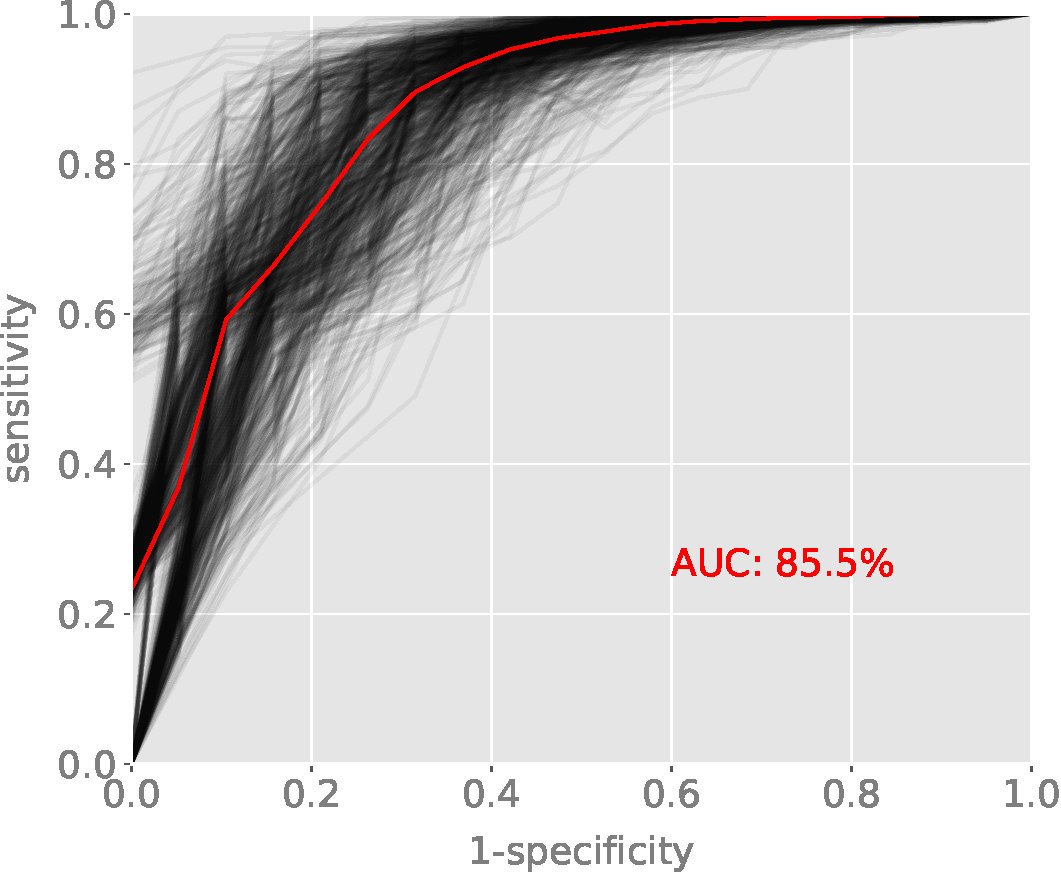
\includegraphics[width=\WDT]{Figures/sczVscaff.pdf}};
\node[anchor=north] (c) at ([yshift=-.3in]a.south) {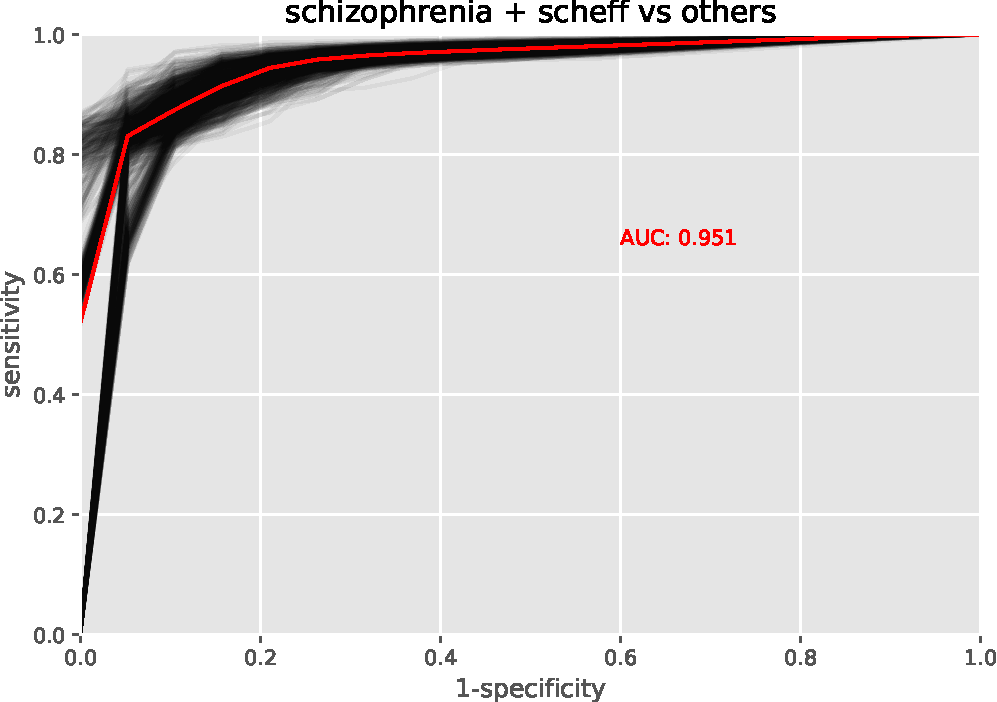
\includegraphics[width=\WDT]{Figures/sczsceff.pdf}};
\node[anchor=south west] (L1) at (a.north west) {{\Large a.} Schizophrenia vs others};
\node[anchor=south west] (L2) at (b.north west) {{\Large b.} Schizophrenia vs Schizoaffective};
\node[anchor=south west] (L3) at (c.north west) {{\Large c.} Schizophrenia or Schizoaffective vs others};

\node[anchor=north west] (T) at ($(c.north west)!(b.west)!(c.north east)$) {
  \mnp{5in}{
\begin{tabular}{L{.65in}|L{.5in}|L{.5in}|L{.5in}|L{.5in}}\hline
 Problem & Confidence & Lower & Upper & Mean \\\hline
SCZ vs SAFF&0.99&0.83&0.88&0.85\\\hline
SCZ vs REST&0.99&0.84&0.87&0.86\\\hline
SCZ+SAFF vs REST&0.99&0.92&0.94&0.93\\\hline
\end{tabular}

  }
};

\node[anchor=south west] (L4) at (T.north west) {{\Large d.} AUC at $99\%$ Confidence};

\end{tikzpicture}

\end{document}
%------------------------------------------------------
\def\TEXTCOL{gray} % all text in the axes and labels
\def\ZCOLA{black} % all text in the axes and labels
\def\ZCOLAm{black!40} % all text in the axes and labels
\def\ZCOLB{Orchid3} % all text in the axes and labels
\def\ZCOLC{teal!80} % all text in the axes and labels

\tikzexternaldisable

\begin{figure}
  \begin{tikzpicture}[font=\bf\sffamily\fontsize{8}{8}\selectfont]
    \def\DATA{qvwho.csv} %define datafile

    \def\WDT{3in} % width 
    \def\HGT{1.5in} % height
    \begin{semilogyaxis}[\TEXTCOL, legend style={text=black,anchor=east,at={(.8,0.8)},
        inner sep=1pt,draw=none,fill=black!5,fill opacity=.75,align=right,
        text opacity=1},
      name=A,
      % at=(F.south west),
      xshift=0in,
      yshift=-0.1in,
      anchor=center,
      width=\WDT,
      height=\HGT,
      scale only axis=true,
      enlargelimits=false,
      enlarge y limits=0.1,
      enlarge x limits=0.04,
      axis on top=false,
      axis line style={black!2, very thick},
      grid,
      grid style={opacity=.95,dashed,ultra thick,black!10},
      % xmin=2001,
      major tick length=0pt,
      ytick style={draw=none},
      scaled y ticks = false,
      y tick label style={/pgf/number format/fixed,
        /pgf/number format/1000 sep = \empty % \thinspace optional
      },
      x tick label style={/pgf/number format/fixed,
        /pgf/number format/1000 sep = \empty % Optional
      },
      ylabel={distance},xlabel={year},
      skip coords between index={0}{1}]
      % add as many addplot commands as u want (draws on same axes)
      \addplot [smooth,
      draw=\ZCOLA, ultra thick,mark=*,
      mark options={scale=2.2,fill=\ZCOLAm,draw=white}]
      table [col sep=comma,x=year,y=lmetric] {\DATA};
      \addlegendentry{lmetric}

    \end{semilogyaxis}
  \end{tikzpicture}
\captionN{Line plot. style 1}
\end{figure}


\begin{figure}
\tikzexternaldisable
  \begin{tikzpicture}[font=\bf\sffamily\fontsize{8}{8}\selectfont]
    \def\DATA{qvwho.csv}
    \def\WDT{3in}
    \def\HGT{1.5in}
    \begin{semilogyaxis}[\TEXTCOL, legend style={text=black,anchor=east,at={(.8,0.8)},
        inner sep=1pt,draw=none,fill=black!5,fill opacity=.75,align=right,
        text opacity=1},
      name=A,
      % at=(F.south west),
      xshift=0in,
      yshift=-0.1in,
      anchor=center,
      width=\WDT,
      height=\HGT,
      scale only axis=true,
      enlargelimits=false,
      enlarge y limits=0.1,
      enlarge x limits=0.04,
      axis on top=false,
      axis line style={black!2, very thick},
      grid,
      grid style={opacity=.95,dashed,ultra thick,black!10},
      % xmin=2001,
      major tick length=0pt,
      ytick style={draw=none},
      scaled y ticks = false,
      y tick label style={/pgf/number format/fixed,
        /pgf/number format/1000 sep = \empty % \thinspace optional
      },
      x tick label style={/pgf/number format/fixed,
        /pgf/number format/1000 sep = \empty % Optional
      },
      ylabel={distance},xlabel={year},
      skip coords between index={0}{1}]
      \addplot [smooth,
      draw=\ZCOLA, ultra thick,,mark=none,mark options={scale=2.2,fill=gray,draw=white}]table [col sep=comma,x=year,y=lmetric] {\DATA};
      \addlegendentry{lmetric}
      \addplot [smooth,
      draw=\ZCOLB, ultra thick,,mark=none,mark options={scale=2.2,fill=gray,draw=white}]table [col sep=comma,x=year,y=qmetric] {\DATA};
      \addlegendentry{qmetric}
    \end{semilogyaxis}
  \end{tikzpicture}
\captionN{Line plot. style 2}
\end{figure}





\begin{figure}

  \begin{tikzpicture}[font=\bf\sffamily\fontsize{8}{8}\selectfont]
    \def\DATA{qvwho.csv}
    \def\WDT{3in}
    \def\HGT{1.5in}
    \begin{axis}[ , legend style={text=black,anchor=east,at={(.8,0.8)},
        inner sep=1pt,draw=none,fill=black!5,fill opacity=.75,align=right,
        text opacity=1},
      name=A,
      xshift=0in,
      yshift=-0.1in,
      anchor=center,
      width=\WDT,
      height=\HGT,
      scale only axis=true,
      enlarge x limits=0.0325,
      axis on top=false,
      axis line style={black!2, ultra thick},
      grid,
      xmin=2001,
      xmax=2018,
      grid style={opacity=.95,dashed,ultra thick,black!10},
      % xticklabel style={xshift=0.05in,yshift=-.05in},
      xlabel style={yshift=.05in,text=\TEXTCOL},
      ylabel style={align=center,,text=\TEXTCOL,anchor=center,
        yshift=-.175in},
      % tickpos=left,
      ytick align=outside,
      xtick align=outside,
      major tick length=0pt,
      scaled y ticks = false,
      y tick label style={/pgf/number format/fixed,
        /pgf/number format/1000 sep = \thinspace % Optional 
      },
      x tick label style={/pgf/number format/fixed,
        /pgf/number format/1000 sep = \thinspace % Optional  
      },
      ylabel={distance},xlabel={year},ybar]

      \addplot [fill=\ZCOLC,draw=none]table [col sep=comma,x=year,y=lmetric] {\DATA};
      \addlegendentry{lmetric}
    \end{axis}
  \end{tikzpicture}
  \caption{barplot}
\end{figure}




\begin{figure}
\centering

  \begin{tikzpicture}[font=\bf\sffamily\fontsize{8}{8}\selectfont]
    \def\DATA{qvwho.csv}
    \def\WDT{2in}
    \def\HGT{.5in}
    \begin{groupplot}[group style={group name=A,group size= 1 by 15,horizontal sep=.5in,vertical sep=.05in},, legend style={text=black,anchor=east,at={(1,0.8)},
        inner sep=1pt,draw=none,fill=black!5,fill opacity=.75,align=right,
        text opacity=1},
      anchor=center,
      width=\WDT,
     height=\HGT,
      scale only axis=true,
      enlarge x limits=0.0325,
      axis on top=false,
      axis line style={black!2, ultra thick},
      grid,
      xmin=2001,
      xmax=2018,
      grid style={opacity=.95,dashed,ultra thick,black!10},
      % xticklabel style={xshift=0.05in,yshift=-.05in},
      xlabel style={yshift=.05in,text=\TEXTCOL},
      ylabel style={align=center,,text=\TEXTCOL,anchor=center,
        yshift=-.175in},
      % tickpos=left,
      ytick align=outside,
      xtick align=outside,
      major tick length=0pt,
      scaled y ticks = false,
      y tick label style={/pgf/number format/fixed,
        /pgf/number format/1000 sep = \thinspace % Optional 
      },
      x tick label style={/pgf/number format/fixed,
        /pgf/number format/1000 sep = \thinspace % Optional  
      },      ylabel={distance},xlabel={year},]
      
      \nextgroupplot[ ybar,xticklabels=\empty,xlabel={},ylabel={},bar width=7pt, ]
      \addplot [fill=\ZCOLC,draw=none]table [col sep=comma,x=year,y=lmetric] {\DATA};
      \addlegendentry{lmetric}

      \nextgroupplot[ ybar,xticklabels=\empty,xlabel={},bar width=7pt, ]
      \addplot [fill=\ZCOLC,draw=none]table [col sep=comma,x=year,y=lmetric] {\DATA};
      \addlegendentry{lmetric}

      \nextgroupplot[ ybar,xticklabels=\empty,xlabel={},bar width=7pt, ]
      \addplot [fill=\ZCOLC,draw=none]table [col sep=comma,x=year,y=lmetric] {\DATA};
      \addlegendentry{lmetric}

      \nextgroupplot[ ybar,xticklabels=\empty,xlabel={},bar width=7pt, ]
      \addplot [fill=\ZCOLC,draw=none]table [col sep=comma,x=year,y=lmetric] {\DATA};
      \addlegendentry{lmetric}

      \nextgroupplot[ ybar,xticklabels=\empty,xlabel={},bar width=7pt, ]
      \addplot [fill=\ZCOLC,draw=none]table [col sep=comma,x=year,y=lmetric] {\DATA};
      \addlegendentry{lmetric}

      \nextgroupplot[ ybar,xticklabels=\empty,xlabel={},bar width=7pt, ]
      \addplot [fill=\ZCOLC,draw=none]table [col sep=comma,x=year,y=lmetric] {\DATA};
      \addlegendentry{lmetric}

      \nextgroupplot[ ybar,xticklabels=\empty,xlabel={},bar width=7pt, ]
      \addplot [fill=\ZCOLC,draw=none]table [col sep=comma,x=year,y=lmetric] {\DATA};
      \addlegendentry{lmetric}

      \nextgroupplot[ ybar,xticklabels=\empty,xlabel={},bar width=7pt, ]
      \addplot [fill=\ZCOLC,draw=none]table [col sep=comma,x=year,y=lmetric] {\DATA};
      \addlegendentry{lmetric}

       \nextgroupplot[ ybar,xticklabels=\empty,xlabel={},bar width=7pt, ]
      \addplot [fill=\ZCOLC,draw=none]table [col sep=comma,x=year,y=lmetric] {\DATA};
      \addlegendentry{lmetric}

       \nextgroupplot[ ybar,xticklabels=\empty,xlabel={},bar width=7pt, ]
      \addplot [fill=\ZCOLC,draw=none]table [col sep=comma,x=year,y=lmetric] {\DATA};
      \addlegendentry{lmetric}

       \nextgroupplot[ ybar,xticklabels=\empty,xlabel={},bar width=7pt, ]
      \addplot [fill=\ZCOLC,draw=none]table [col sep=comma,x=year,y=lmetric] {\DATA};
      \addlegendentry{lmetric}

       \nextgroupplot[ ybar,xticklabels=\empty,xlabel={},bar width=7pt, ]
      \addplot [fill=\ZCOLC,draw=none]table [col sep=comma,x=year,y=lmetric] {\DATA};
      \addlegendentry{lmetric}

       \nextgroupplot[ ybar,xticklabels=\empty,xlabel={},bar width=7pt, ]
      \addplot [fill=\ZCOLC,draw=none]table [col sep=comma,x=year,y=lmetric] {\DATA};
      \addlegendentry{lmetric}

       \nextgroupplot[ ybar,xticklabels=\empty,xlabel={},bar width=7pt, ]
      \addplot [fill=\ZCOLC,draw=none]table [col sep=comma,x=year,y=lmetric] {\DATA};
      \addlegendentry{lmetric}

      \nextgroupplot[ ybar,ylabel={},bar width=7pt, ]
      \addplot [fill=\ZCOLC,draw=none]table [col sep=comma,x=year,y=lmetric] {\DATA};
      \addlegendentry{lmetric}


    \end{groupplot}

  \end{tikzpicture}
  \caption{group plot example}
\end{figure}


\end{document}



